
%(BEGIN_QUESTION)
% Copyright 2010, Tony R. Kuphaldt, released under the Creative Commons Attribution License (v 1.0)
% This means you may do almost anything with this work of mine, so long as you give me proper credit

This liquid level control system uses two split-ranged control valves to either add liquid to the vessel (LV-37a) or drain liquid from it (LV-37b), depending on which action is necessary to hold the level at setpoint:

$$\includegraphics[width=15.5cm]{i04459x01.eps}$$

Suppose one day the operator calls you to complain that the liquid level inside this vessel registers about 40\% on the controller faceplate and has been for at least a full day, with a constant setpoint of 50\%.  The operator has not gone to the actual vessel to verify the real level.  Based on this single symptom, identify the likelihood of each of the following faults considered one at a time (i.e. no coincidental faults) being able to account for the high (indicated) liquid level.  Simply write a check mark in the appropriate box (either ``possible'' or ``impossible'') for each proposed fault:

% No blank lines allowed between lines of an \halign structure!
% I use comments (%) instead, so that TeX doesn't choke.

$$\vbox{\offinterlineskip
\halign{\strut
\vrule \quad\hfil # \ \hfil & 
\vrule \quad\hfil # \ \hfil & 
\vrule \quad\hfil # \ \hfil \vrule \cr
\noalign{\hrule}
%
% First row
{\bf Fault} & {\bf Possible} & {\bf Impossible} \cr
%
\noalign{\hrule}
%
% Another row
Level transmitter registering too low &  & \cr
%
\noalign{\hrule}
%
% Another row
Level transmitter registering too high &  & \cr
%
\noalign{\hrule}
%
% Another row
Valve LV-37a stuck open &  &  \cr
%
\noalign{\hrule}
%
% Another row
Cable from LIC-37 to LV-37a failed open &  & \cr
%
\noalign{\hrule}
%
% Another row
Cable from LIC-37 to LV-37a failed shorted &  & \cr
%
\noalign{\hrule}
%
% Another row
Cable from LIC-37 to LV-37b failed open &  & \cr
%
\noalign{\hrule}
%
% Another row
Cable from LIC-37 to LV-37b failed shorted &  & \cr
%
\noalign{\hrule}
%
% Another row
Controller configured for P-only action &  & \cr
%
\noalign{\hrule}
%
% Another row
Controller configured for I-only action &  & \cr
%
\noalign{\hrule}
%
% Another row
PID controller configured for direct action &  & \cr
%
\noalign{\hrule}
} % End of \halign 
}$$ % End of \vbox

\underbar{file i04459}
%(END_QUESTION)





%(BEGIN_ANSWER)

% No blank lines allowed between lines of an \halign structure!
% I use comments (%) instead, so that TeX doesn't choke.

$$\vbox{\offinterlineskip
\halign{\strut
\vrule \quad\hfil # \ \hfil & 
\vrule \quad\hfil # \ \hfil & 
\vrule \quad\hfil # \ \hfil \vrule \cr
\noalign{\hrule}
%
% First row
{\bf Fault} & {\bf Possible} & {\bf Impossible} \cr
%
\noalign{\hrule}
%
% Another row
Level transmitter registering too low &  & $\surd$ \cr
%
\noalign{\hrule}
%
% Another row
Level transmitter registering too high &  & $\surd$ \cr
%
\noalign{\hrule}
%
% Another row
Valve LV-37a stuck open &  & $\surd$ \cr
%
\noalign{\hrule}
%
% Another row
Cable from LIC-37 to LV-37a failed open & $\surd$  & \cr
%
\noalign{\hrule}
%
% Another row
Cable from LIC-37 to LV-37a failed shorted & $\surd$  & \cr
%
\noalign{\hrule}
%
% Another row
Cable from LIC-37 to LV-37b failed open &  & $\surd$ \cr
%
\noalign{\hrule}
%
% Another row
Cable from LIC-37 to LV-37b failed shorted &  & $\surd$ \cr
%
\noalign{\hrule}
%
% Another row
Controller configured for P-only action & $\surd$ & \cr
%
\noalign{\hrule}
%
% Another row
Controller configured for I-only action &  & $\surd$ \cr
%
\noalign{\hrule}
%
% Another row
PID controller configured for direct action &  & $\surd$ \cr
%
\noalign{\hrule}
} % End of \halign 
}$$ % End of \vbox


%(END_ANSWER)





%(BEGIN_NOTES)

{\bf This question is intended for exams only and not worksheets!}.

%(END_NOTES)

